%!TEX TS-program = xelatex
\documentclass[11pt]{article}

\usepackage[english]{babel}

\usepackage{amsmath,amssymb,amsfonts}
\usepackage[utf8]{inputenc}
\usepackage[T1]{fontenc}
\usepackage{stix2}
\usepackage[scaled]{helvet}
\usepackage[scaled]{inconsolata}

\usepackage{lastpage}

\usepackage{setspace}

\usepackage{ccicons}

\usepackage[hang,flushmargin]{footmisc}

\usepackage{geometry}

\setlength{\parindent}{0pt}
\setlength{\parskip}{6pt plus 2pt minus 1pt}

\usepackage{fancyhdr}
\renewcommand{\headrulewidth}{0pt}\providecommand{\tightlist}{%
  \setlength{\itemsep}{0pt}\setlength{\parskip}{0pt}}

\makeatletter
\newcounter{tableno}
\newenvironment{tablenos:no-prefix-table-caption}{
  \caption@ifcompatibility{}{
    \let\oldthetable\thetable
    \let\oldtheHtable\theHtable
    \renewcommand{\thetable}{tableno:\thetableno}
    \renewcommand{\theHtable}{tableno:\thetableno}
    \stepcounter{tableno}
    \captionsetup{labelformat=empty}
  }
}{
  \caption@ifcompatibility{}{
    \captionsetup{labelformat=default}
    \let\thetable\oldthetable
    \let\theHtable\oldtheHtable
    \addtocounter{table}{-1}
  }
}
\makeatother

\usepackage{array}
\newcommand{\PreserveBackslash}[1]{\let\temp=\\#1\let\\=\temp}
\let\PBS=\PreserveBackslash

\usepackage[breaklinks=true]{hyperref}
\hypersetup{colorlinks,%
citecolor=blue,%
filecolor=blue,%
linkcolor=blue,%
urlcolor=blue}
\usepackage{url}

\usepackage{caption}
\setcounter{secnumdepth}{0}
\usepackage{cleveref}

\usepackage{graphicx}
\makeatletter
\def\maxwidth{\ifdim\Gin@nat@width>\linewidth\linewidth
\else\Gin@nat@width\fi}
\makeatother
\let\Oldincludegraphics\includegraphics
\renewcommand{\includegraphics}[1]{\Oldincludegraphics[width=\maxwidth]{#1}}

\usepackage{longtable}
\usepackage{booktabs}

\usepackage{color}
\usepackage{fancyvrb}
\newcommand{\VerbBar}{|}
\newcommand{\VERB}{\Verb[commandchars=\\\{\}]}
\DefineVerbatimEnvironment{Highlighting}{Verbatim}{commandchars=\\\{\}}
% Add ',fontsize=\small' for more characters per line
\usepackage{framed}
\definecolor{shadecolor}{RGB}{248,248,248}
\newenvironment{Shaded}{\begin{snugshade}}{\end{snugshade}}
\newcommand{\KeywordTok}[1]{\textcolor[rgb]{0.13,0.29,0.53}{\textbf{#1}}}
\newcommand{\DataTypeTok}[1]{\textcolor[rgb]{0.13,0.29,0.53}{#1}}
\newcommand{\DecValTok}[1]{\textcolor[rgb]{0.00,0.00,0.81}{#1}}
\newcommand{\BaseNTok}[1]{\textcolor[rgb]{0.00,0.00,0.81}{#1}}
\newcommand{\FloatTok}[1]{\textcolor[rgb]{0.00,0.00,0.81}{#1}}
\newcommand{\ConstantTok}[1]{\textcolor[rgb]{0.00,0.00,0.00}{#1}}
\newcommand{\CharTok}[1]{\textcolor[rgb]{0.31,0.60,0.02}{#1}}
\newcommand{\SpecialCharTok}[1]{\textcolor[rgb]{0.00,0.00,0.00}{#1}}
\newcommand{\StringTok}[1]{\textcolor[rgb]{0.31,0.60,0.02}{#1}}
\newcommand{\VerbatimStringTok}[1]{\textcolor[rgb]{0.31,0.60,0.02}{#1}}
\newcommand{\SpecialStringTok}[1]{\textcolor[rgb]{0.31,0.60,0.02}{#1}}
\newcommand{\ImportTok}[1]{#1}
\newcommand{\CommentTok}[1]{\textcolor[rgb]{0.56,0.35,0.01}{\textit{#1}}}
\newcommand{\DocumentationTok}[1]{\textcolor[rgb]{0.56,0.35,0.01}{\textbf{\textit{#1}}}}
\newcommand{\AnnotationTok}[1]{\textcolor[rgb]{0.56,0.35,0.01}{\textbf{\textit{#1}}}}
\newcommand{\CommentVarTok}[1]{\textcolor[rgb]{0.56,0.35,0.01}{\textbf{\textit{#1}}}}
\newcommand{\OtherTok}[1]{\textcolor[rgb]{0.56,0.35,0.01}{#1}}
\newcommand{\FunctionTok}[1]{\textcolor[rgb]{0.00,0.00,0.00}{#1}}
\newcommand{\VariableTok}[1]{\textcolor[rgb]{0.00,0.00,0.00}{#1}}
\newcommand{\ControlFlowTok}[1]{\textcolor[rgb]{0.13,0.29,0.53}{\textbf{#1}}}
\newcommand{\OperatorTok}[1]{\textcolor[rgb]{0.81,0.36,0.00}{\textbf{#1}}}
\newcommand{\BuiltInTok}[1]{#1}
\newcommand{\ExtensionTok}[1]{#1}
\newcommand{\PreprocessorTok}[1]{\textcolor[rgb]{0.56,0.35,0.01}{\textit{#1}}}
\newcommand{\AttributeTok}[1]{\textcolor[rgb]{0.77,0.63,0.00}{#1}}
\newcommand{\RegionMarkerTok}[1]{#1}
\newcommand{\InformationTok}[1]{\textcolor[rgb]{0.56,0.35,0.01}{\textbf{\textit{#1}}}}
\newcommand{\WarningTok}[1]{\textcolor[rgb]{0.56,0.35,0.01}{\textbf{\textit{#1}}}}
\newcommand{\AlertTok}[1]{\textcolor[rgb]{0.94,0.16,0.16}{#1}}
\newcommand{\ErrorTok}[1]{\textcolor[rgb]{0.64,0.00,0.00}{\textbf{#1}}}
\newcommand{\NormalTok}[1]{#1}

\newlength{\cslhangindent}
\setlength{\cslhangindent}{1.5em}
\newlength{\csllabelwidth}
\setlength{\csllabelwidth}{3em}
\newenvironment{CSLReferences}[3] % #1 hanging-ident, #2 entry spacing
 {% don't indent paragraphs
  \setlength{\parindent}{0pt}
  % turn on hanging indent if param 1 is 1
  \ifodd #1 \everypar{\setlength{\hangindent}{\cslhangindent}}\ignorespaces\fi
  % set entry spacing
  \ifnum #2 > 0
  \setlength{\parskip}{#2\baselineskip}
  \fi
 }%
 {}
\usepackage{calc} % for \widthof, \maxof
\newcommand{\CSLBlock}[1]{#1\hfill\break}
\newcommand{\CSLLeftMargin}[1]{\parbox[t]{\maxof{\widthof{#1}}{\csllabelwidth}}{#1}}
\newcommand{\CSLRightInline}[1]{\parbox[t]{\linewidth}{#1}}
\newcommand{\CSLIndent}[1]{\hspace{\cslhangindent}#1}\geometry{verbose,letterpaper,tmargin=2.2cm,bmargin=2.2cm,lmargin=2.2cm,rmargin=2.2cm}

\usepackage{lineno}
\usepackage[nolists,noheads]{endfloat}

\pagestyle{plain}

\tolerance=1
\emergencystretch=\maxdimen
\hyphenpenalty=10000
\hbadness=10000

\doublespacing

\fancypagestyle{normal}
{
  \fancyhf{}
  \fancyfoot[R]{\footnotesize\sffamily\thepage\ of \pageref*{LastPage}}
}
\begin{document}
\raggedright
\thispagestyle{empty}
{\Large\bfseries\sffamily Dissimilarity of species interaction networks:
quantifying the effect of turnover and rewiring}
\vskip 5em

%
\href{https://orcid.org/0000-0002-0735-5184}{Timothée\,Poisot}%
%
\,\textsuperscript{1,2,‡}

\textsuperscript{1}\,Université de
Montréal\quad \textsuperscript{2}\,Québec Centre for Biodiversity
Sciences

\textsuperscript{‡}\,These authors contributed equally to the work\\

\textbf{Correspondance to:}\\
Timothée Poisot --- \texttt{timothee.poisot@umontreal.ca}\\

\vfill
This work is released by its authors under a CC-BY 4.0 license\hfill\ccby\\
Last revision: \emph{\today}

\clearpage
\thispagestyle{empty}

\vfill
Despite having established its usefulness in the last ten years, the
decomposition of ecological networks in components allowing to measure
their \(\beta\)-diversity retains some methodological ambiguities.
Notably, how to quantify the relative effect of mechanisms tied to
interaction rewiring \emph{vs.} species turnover has been interpreted
differently by different authors. In this contribution, I present
mathematical arguments and numerical experiments that should (i)
establish that the decomposition of networks as it is currently done is
indeed fit for purpose, and (ii) provide guidelines to interpret the
values of the components tied to turnover and rewiring.



\vfill

\clearpage
\linenumbers
\pagestyle{normal}

Ecological networks are variable both in time and space (Poisot \emph{et
al.} 2015; Trøjelsgaard \& Olesen 2016) - this variability motivated the
emergence of methodology to compare ecological networks, including in a
way that meshes with the core concept for the comparison of ecological
communities, namely \(\beta\)-diversity (Poisot \emph{et al.} 2012). The
need to understand network variability through partitioning in
components equivalent to \(\alpha\), \(\beta\), and \(\gamma\)
diversities is motivated by the prospect to further integrate the
analysis of species interactions to the analysis of species
compositions. Because species that make up the networks do not react to
their environment in the same way, and because interactions are only
expressed in subsets of the environments in which species co-occurr, the
\(\beta\)-diversity of networks may behave in complex ways, and its
quantification is likely to be ecologically informative.

Poisot \emph{et al.} (2012) and Canard \emph{et al.} (2014) have
suggested an approach to \(\beta\)-diversity for ecological networks
which is based on the comparison of the number of shared and unique
links among species within a pair of networks. Their approach
differentiates this sharing of links between those established between
species occurring in both networks, and those established with at least
one unique species. This framework is expressed as the decomposition
\(\beta_{wn} = \beta_{os} + \beta_{st}\), namely the fact that network
dissimilarity (\(\beta_{wn}\)) has a component that can be calculated
directly from the dissimilarity of interactions between shared species
(\(\beta_{os}\)), and a component that cannot (\(\beta_{st}\)).
Presumably, the value of these components for a pair of networks can
generate insights about the mechanisms involved in dissimilarity.

This approach has been widely adopted since its publication, with recent
examples using it to understand the effect of fire on pollination
systems (Baronio \emph{et al.} 2021); the impact of rewiring on
spatio-temporal network dynamics (Campos-Moreno \emph{et al.} 2021); the
effects of farming on rural and urban landscapes on species interactions
(Olsson \emph{et al.} 2021); the impact of environment gradients on
multi-trophic metacommunities (\textbf{Ohlmann2018MapImp?}); and as a
tool to estimate the sampling completeness of networks (Souza \emph{et
al.} 2021). It has, similarly, received a number of extensions,
including the ability to account for interaction strength (Magrach
\emph{et al.} 2017), the ability to handle probabilistic ecological
networks (Poisot \emph{et al.} 2016), and the integration into the Local
Contribution to Beta Diversity (Legendre \& De Cáceres 2013) approach to
understand how environment changes drive network dissimilarity (Poisot
\emph{et al.} 2017).

\begin{figure}
\hypertarget{fig:conceptual}{%
\centering
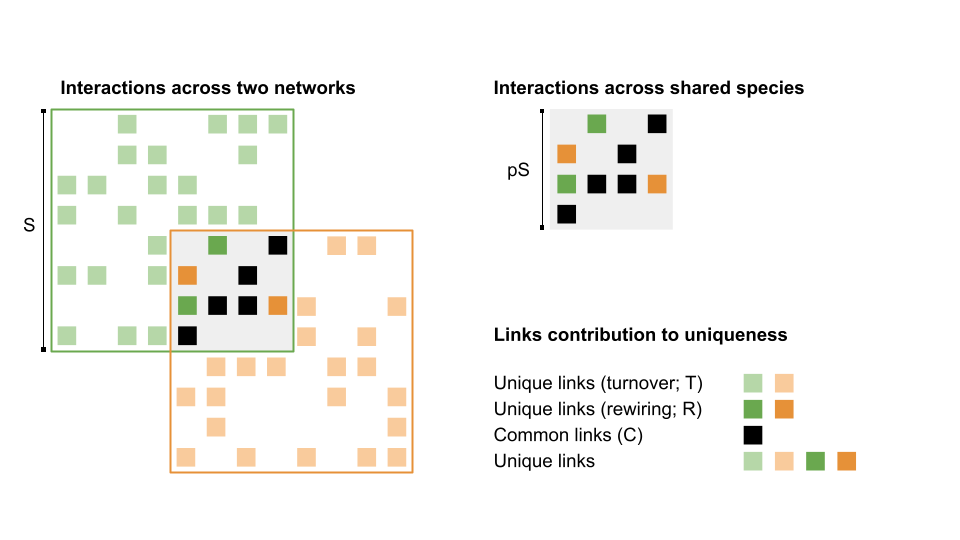
\includegraphics{figures/betadiv_response_figure.png}
\caption{The dissimilarity of two networks (green and orange) of equal
richness \(S\) (this also holds for unequal richness) depends on three
families of interactions: those that are unique because of species
turnover (in a pale color), those that are unique because of rewiring
(in a saturated color), and those that are shared (in black). Assuming
that the chance of sharing a species between the two networks is \(p\),
then there can be at most \(p^2\times S^2\) shared links -- for this
reason, overall network dissimilarity (\(\beta_{wn}\)) will have a
component tied to species turnover, which is
\(\beta_{st}\).}\label{fig:conceptual}
}
\end{figure}

Yet, the precise meaning of \(\beta_{st}\), namely the importance of
species turnover in the overall dissimilarity, has been difficult to
capture, and a source of confusion for some practitioners. This is not
particularly surprising, as this component of the decomposition responds
to unique species introducing their unique interactions both between
themselves, and with species that are common to both networks
fig.~\ref{fig:conceptual}. For this reason, it is important to come up
with guidelines for the interpretation of this measure, and how to use
it to extract ecological insights.

Furthermore, much like the definition of \(\beta\)-diversity in all its
forms is a contentious topic amongst community ecologists (see
\emph{e.g.} Tuomisto 2010), the \(\beta\)-diversity of networks has been
submitted to methodological scrutiny over the years. A synthesis of some
criticisms, related to the correct denominator to use to express the
proportion of different links, has recently been published (Fründ 2021).
It argues that the calculation of network dissimilarity terms as
originally outlined by Poisot \emph{et al.} (2012) is incorrect, as it
can lead to over-estimating the role of interactions between shared
species in a network (``rewiring''), and therefore underestimate the
importance of species turnover across networks. As mist-understanding
either of these quantities can lead to biased inferences about the
mechanisms generating network dissimilarity, it is important to assess
how the values (notably of \(\beta_{os}\), and therefore of
\(\beta_{st}\)) react to methodological choices.

Here, I present a mathematical analysis of the Poisot \emph{et al.}
(2012) method, explain how information about species turnover and link
rewiring can be extracted from its decomposition, and conduct numerical
experiments to guide the interpretation of the \(\beta\)-diversity
values thus obtained (with a specific focus on \(\beta_{st}\)). These
numerical experiments establish three core facts. First, the
decomposition adequately captures the relative roles of species turnover
and interaction rewiring; second, the decomposition responds to
differences in network structure (like connectance) as expected;
finally, the decomposition more accurately captures rewiring than the
proposed alternative using a different denominator put forth by Fründ
(2021).

\hypertarget{partitioning-network-dissimilarity}{%
\subsection{Partitioning network
dissimilarity}\label{partitioning-network-dissimilarity}}

The approach to quantifying the difference between pairs of networks
established in Poisot \emph{et al.} (2012) is a simple extension of the
overall method by Koleff \emph{et al.} (2003) for species dissimilarity
based on presence-absence data. The objects to compare, \(X_1\) and
\(X_2\), are partitioned into three values, \(a = |X_1 \cup X_2|\),
\(b = |X_2 \setminus X_1|\), and \(c = |X_1 \setminus X_2|\), where
\(|\cdot|\) is the cardinality of set \(\cdot\) (the number of elements
it contains), and \(\setminus\) is the set substraction operation. In
the perspective of species composition comparison, \(X_1\) and \(X_2\)
are the sets of species in either community, so that if
\(X_1 = \{x, y, z\}\) and \(X_2 = \{v, w, x, y\}\), we have
\(X_1 \cup X_2 = \{v, w, x, y, z\}\), \(X_1 \cap X_2 = \{x, y\}\),
\(X_2 \setminus X_1 = \{v, w\}\), and \(X_1 \setminus X_2 = \{z\}\). The
core message of Koleff \emph{et al.} (2003) is that the overwheling
majority of measures of \(\beta\)-diversity can be re-expressed as
functions that operate on the cardinality of these sets -- this allows
to focus on the number of unique and common elements, as outlined in
fig.~\ref{fig:conceptual}.

\hypertarget{re-expressing-networks-as-sets}{%
\subsubsection{Re-expressing networks as
sets}\label{re-expressing-networks-as-sets}}

Applying this framework to networks requires a few additional
definitions. Although ecologists tend to think of networks as their
adjacency matrix (as is presented in fig.~\ref{fig:conceptual}), this
representation is not optimal to reach a robust understanding of which
elements should be counted as part of which set when measuring network
dissimilarity. For this reason, we need fall back on the definition of a
graph as a pair of sets, wherein \(\mathcal{G} = (V, E)\). These two
components \(V\) and \(E\) represent vertices (nodes, species) and edges
(interactions), where \(V\) is specifically a set containing the
vertices of \(\mathcal{G}\), and \(E\) is a set of ordered pairs, in
which every pair is composed of two elements of \(V\); an element
\(\{i,j\}\) in \(E\) indicates that there is an interaction \emph{from}
species \(i\) to species \(j\) in the network \(\mathcal{G}\). The
adjancency matrix \(\mathbf{A}\) of this network would therefore have a
non-zero entry at \(A_{ij}\).

In the context of networks comparison (assuming the networks to compare
are \(\mathcal{M}\) and \(\mathcal{N}\)), we can further decompose the
contents of these sets as

\[\mathcal{M} = (V_c \cup V_m, E_c \cup E_{sm} \cup E_{um}) \,,\]

and

\[\mathcal{N} = (V_c \cup V_n, E_c \cup E_{sn} \cup E_{un}) \,,\]

where \(V_c\) is the set of common species, \(V_m\) and \(V_n\) are the
species belonging only to network \(m\) and \(n\) (respectively),
\(E_c\) are the common edges, and \(E_{sm}\) and \(E_{um}\) are the
interactions unique to \(k\) involving, respectively, only species in
\(V_c\), and at least one species from \(V_m\) (the same notation
applies for the subscript \(_{n}\)).

\hypertarget{defining-the-partitions-from-networks-as-sets}{%
\subsubsection{Defining the partitions from networks as
sets}\label{defining-the-partitions-from-networks-as-sets}}

The metaweb (Dunne 2006), which is to say the entire regional species
pool and their interaction, can be defined as
\(\mathcal{M} \cup \mathcal{N}\) (this operation is commutative), which
is to say

\[\mathcal{M} \cup \mathcal{N} = (V_c \cup V_m \cup V_n, E_c \cup E_{sm} \cup E_{um} \cup E_{sn} \cup E_{un}) \,.\]

This operation gives us an equivalent to \(\gamma\)-diversity for
networks, in that the set of vertices contains \emph{all} species from
the two networks, and the set of edges contains \emph{all} the
interactions between these species. If, further, we make the usual
assumption that only species with at least one interaction are present
in the set of vertices, then all elements of the set of vertices are
present at least once in the set of edges, and the set of vertices can
be entire reconstructed from the set of edges. Although measures of
network \(\beta\)-diversity operate on interactions (not species), this
property is maintained at every decomposition we will describe next.

We can similarly define the intersection (similarly commutative) of two
networks:

\[\mathcal{M} \cap \mathcal{N} = (V_c, E_c)\,.\]

The decomposition of \(\beta\)-diversity from Poisot \emph{et al.}
(2012) uses these components to measure \(\beta_{os}\) (``rewiring''),
and \(\beta_{wn}\) (the overall dissimilarity including non-shared
species). We can express the components \(a\), \(b\), and \(c\) of
Koleff \emph{et al.} (2003) as the cardinality of the following sets:

\begin{longtable}[]{@{}llll@{}}
\toprule
Component & \(a\) & \(b\) & \(c\)\tabularnewline
\midrule
\endhead
\(\beta_{os}\) & \(E_c\) & \(E_{sn}\) & \(E_{sm}\)\tabularnewline
\(\beta_{wn}\) & \(E_c\) & \(E_{sn} \cup E_{un}\) &
\(E_{sm} \cup E_{um}\)\tabularnewline
\bottomrule
\end{longtable}

It is fundamental to note that these components can be measured entirely
from the interactions, and that the number of species in either network
are never directly involved.

In the following sections, I present a series of calculations aimed at
expressing the values of \(\beta_{os}\), \(\beta_{wn}\), and therefore
\(\beta_{st}\) as a function of species sharing probability (as a proxy
for mechanisms generating turnover), and link rewiring probability (as a
proxy for mechanisms generating differences in interactions among shared
species). These calculations are done using \texttt{Symbolics.jl}
(\textbf{Gowda2021HigSym?}), and subsequently transformed in executable
code for \emph{Julia} (\textbf{Bezanson2017JulFre?}), used to produce
the figures.

\hypertarget{quantifying-the-importance-of-species-turnover}{%
\subsubsection{Quantifying the importance of species
turnover}\label{quantifying-the-importance-of-species-turnover}}

The difference between \(\beta_{os}\) and \(\beta_{wn}\) stems from the
species dissimilarity between \(\mathcal{M}\) and \(\mathcal{N}\), and
it is easier to understand the effect of turnover by picking a
dissimilarity measure to work as an exemplar. We will use
\(\beta = (b+c)/(2a+b+c)\), which in the Koleff \emph{et al.} (2003)
framework is (Wilson \& Shmida 1984). This measure returns values in
\([0,1]\), with \(0\) meaning complete similarity, and \(1\) meaning
complete dissimilarity.

Based on a partition between three sets of cardinality \(a\), \(b\), and
\(c\),

\[\beta_t = \frac{b+c}{2a+b+c}\,.\]

So as to simplify the notation of the following section, I will
introduce a series of new variables. Let \(C = |E_c|\) be the number of
links that are identical between networks (as a mnemonic, \(C\) stands
for ``common''); \(R = |E_{sn} \cup E_{sm}|\) be the number of links
that are not shared, but only involve shared species (\emph{i.e.} links
from \(\mathcal{M}\cup\mathcal{N}\) established between species from
\(\mathcal{M}\cap\mathcal{N}\); as a mnemonic, \(R\) stands for
``rewired''); and \(T = |E_{un} \cup E_{um}|\) the number of links that
are not shared, and involve at least one unique species (as a mnemonic,
\(T\) stands for ``turnover'').

There are two important points to note here. First, as mentionned
earlier, the number or proportion of species that are shared is not
involved in the calculation. Second, the connectance of either network
is not involved in the calculation. That all links counted in
\emph{e.g.} \(U\) come from \(\mathcal{M}\), or that they are evenly
distributed between \(\mathcal{M}\) and \(\mathcal{N}\), has no impact
on the result. This is a desirable property of the approach: whatever
quantitative value of the components of dissimilarity can be interpreted
in the light of the connectance and species turnover \emph{without} any
risk of circularity; indeed, I present a numerical experiment where
connectance varies independently later in this manuscript, reinforcing
this point.

The final component of network dissimilarity in Poisot \emph{et al.}
(2012) is \(\beta_{st}\), \emph{i.e.} the part of \(\beta_{wn}\) that is
not explained by changes in interactions between shared species
(\(\beta_{os}\)), and therefore stems from species turnover. This
fraction is defined as \(\beta_{st} = \beta_{wn}-\beta_{os}\). The
expression of \(\beta_{st}\) does not involve a partition into sets that
can be plugged into the framework of Koleff \emph{et al.} (2003),
because the part of \(\mathcal{M}\) and \(\mathcal{N}\) that are
composed of their unique species cannot, by definition, share
interactions. One could, theoretically, express these as
\(\mathcal{M} \setminus \mathcal{N} = (V_m, E_{um})\) and
\(\mathcal{N} \setminus \mathcal{M} = (V_v, E_{un})\) (note the
non-commutativity here), but the dissimilarity between these networks is
trivially maximal for the measures considered.

Using the \(\beta_t\) measure of dissimilarity, we can re-write (using
the notation with \(A\), \(S\), and \(U\))

\[\beta_{os} = \frac{R}{2C+R}\,,\]

and

\[\beta_{wn} = \frac{R+T}{2C+R+T}\,.\]

Note that \(\beta_{os}\) has the form \(x/y\) with \(x = S\) and
\(y = 2A+S\), and \(\beta_{wn}\) has the form \((x+k)/(y+k)\), with
\(k = U\). As long as \(k \ge 0\), it is guaranteed that
\(\beta_{wn} \ge \beta_{os}\), and therefore that
\(0 \ge \beta_{st} \ge 1\); as \(C\), \(T\), and \(R\) are cardinalities
of sets, they are necessarily satisfying this condition.

We can get an expression for \(\beta_{st}\), by bringing \(\beta_{os}\)
and \(\beta_{wn}\) to a common denominator and simplifying the
numerator:

\[\beta_{st} = \frac{2CT}{(2C+R)(2C+R+T)}\,.\]

Note that this value varies in a non-monotonic way with regards to the
number of interactions that are part of the common set of species --
this is obvious when developing the denominator into
\(4C^2 + R^2 + 4CR + 2CT + RT\). As such, we expect that the value of
\(\beta_{st}\) will vary in a hump-shaped way with the proportion of
shared interactions. For this reason, Poisot \emph{et al.} (2012)
suggest that \(\beta_{st}/\beta{wn}\) (alt. \(1-\beta_{os}/\beta_{wn}\))
is a better indicator of the \emph{relative} importance of turnover
processes on network dissimilarity. This can be calculated as

\[\frac{\beta_{st}}{\beta_{wn}} = \frac{2CT}{(2C+S)(2C+R+T)}\times\frac{R+T}{2C+R+T}\,,\]

which reduces to

\[\frac{\beta_{st}}{\beta_{wn}} = \frac{2CT}{(2C+R)(R+T)}\,.\]

The roots of this expression are \(C=0\) (the turnover of species has no
contribution to the difference between \(\beta_{wn}\) and \(\beta_{os}\)
if there are no shared species, and therefore no rewiring), and for
\(T = 0\) (the turnover of species has no contribution if all species
are shared).

\hypertarget{quantifying-the-response-of-network-beta-diversity-to-souces-of-variation}{%
\subsection{Quantifying the response of network beta-diversity to souces
of
variation}\label{quantifying-the-response-of-network-beta-diversity-to-souces-of-variation}}

\hypertarget{the-relative-effect-of-species-turnover-and-link-rewiring}{%
\subsubsection{The relative effect of species turnover and link
rewiring}\label{the-relative-effect-of-species-turnover-and-link-rewiring}}

As the decomposition of beta diversity into sets presented above
reveals, the value of the components \(\beta_{os}\) and \(\beta_{st}\)
will respond to two family of mechanisms: the probability of sharing a
species between the two networks, noted \(p\), which will impose bounds
on the value of \(T\); and the probability of an interactions between
shared species \emph{not} being rewired, noted \(q\), which will impose
bounds on the value of \(C\). These two probabilities represent,
respectively, mechanisms involved in species turnover and link turnover,
as per Poisot \emph{et al.} (2015), and the aim of this numerical
experiment is to describe how these families of processes drive network
dissimilarity.

In order to simplify the calculations, I make the assumptions that the
networks have equal species richness (noted \(S\)), so that
\(S_1 = S_2 = S\), and the same connectance (noted \(\rho\)), so that
\(\rho_1 = \rho_2 = \rho\). As a consequence, the two networks have the
same number of links \(L = \rho\times S_1^2 = \rho\times S_2^2\). The
assumption of equal connectance will be relaxed in a subsequent
numerical experiment. These simplifications allow to express the size of
\(C\), \(R\), and \(T\) only as functions of \(p\) and \(q\), as they
would all be multiplied by \(L\), which can therefore be dropped from
the calculation.

\begin{figure}
\hypertarget{fig:turnrew}{%
\centering
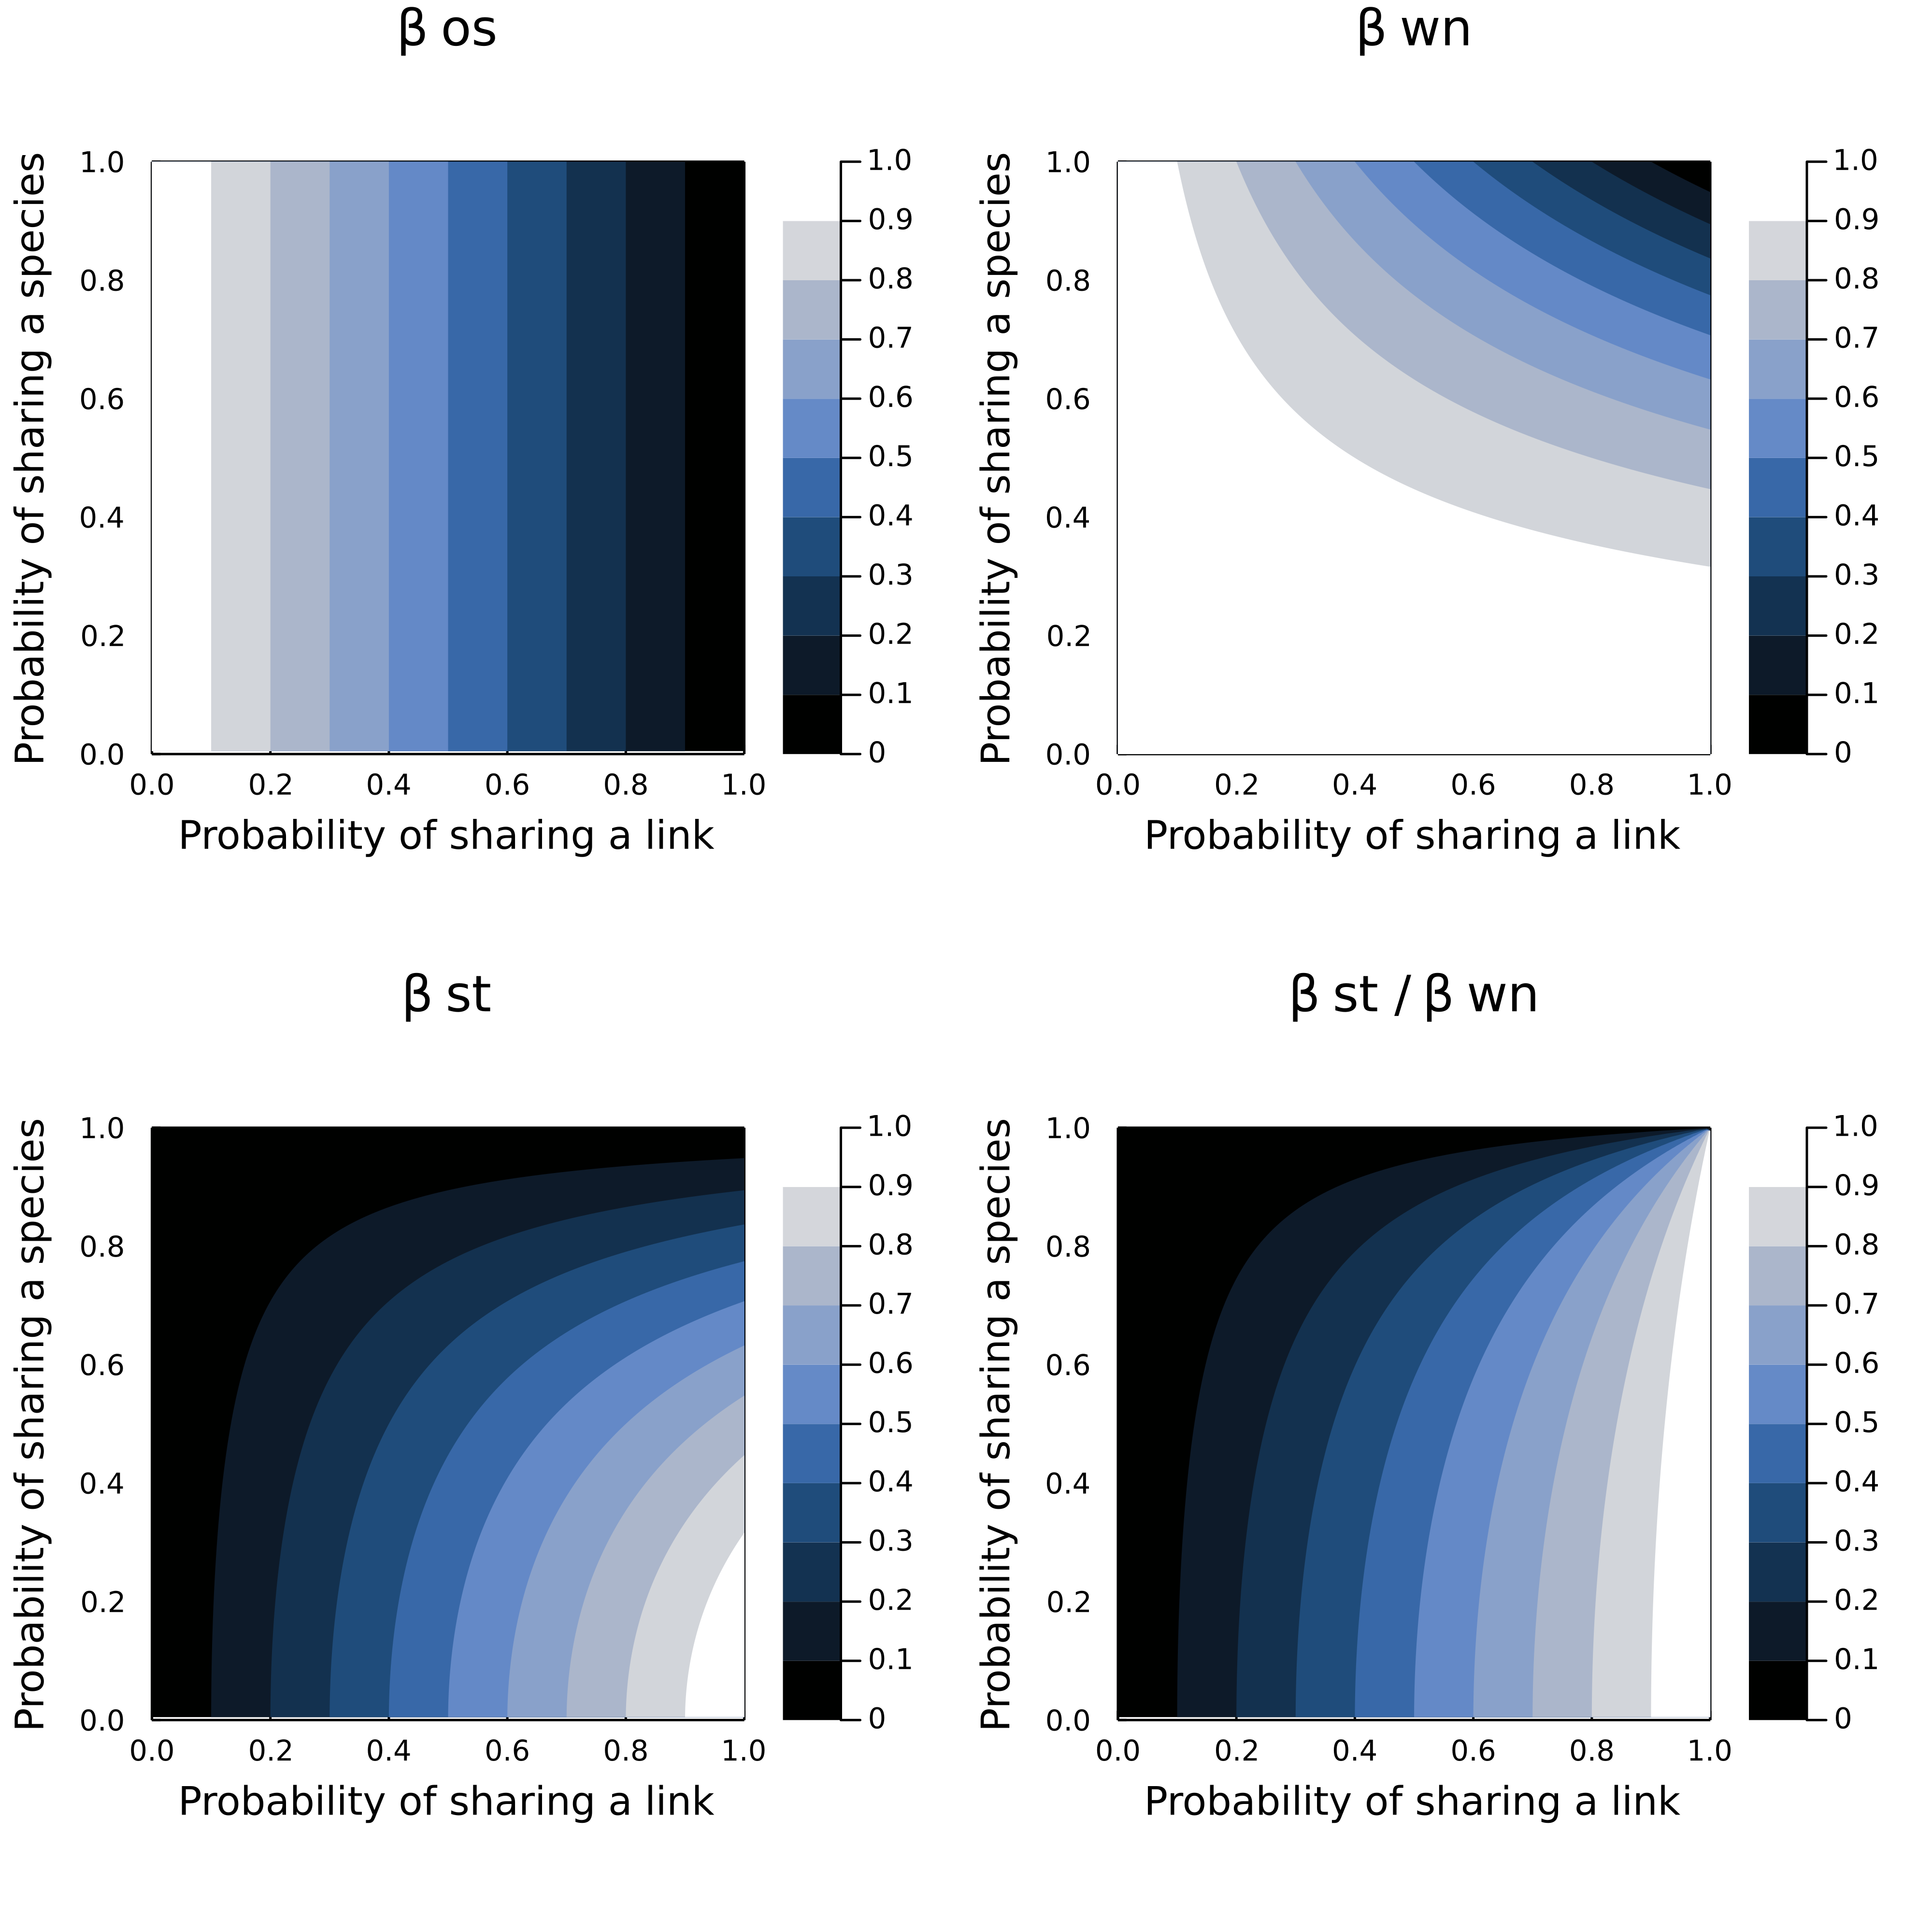
\includegraphics{figures/sharing_v_rewiring/components.png}
\caption{Values of \(\beta_{os}\), \(\beta_{wn}\), \(\beta_{st}\), and
\(\beta_{st}/\beta_{wn}\) as a function of the probability \(q\) or
sharing a link (\(x\)-axis), and the probability \(p\) of sharing a
species (\(y\)-axis). Larger values indicate \emph{more} dissimilarity,
such that for \(p=q=1\) the dissimilarity as measured by
\(\beta_{wn}=0\), and for \(p=q=0\) the dissimilarity as measured by
\(\beta_{wn}=1\). As expected, the relative importance of turnover
(\(\beta_{st}\)) is maximal when there is no rewiring, and when turnover
increases.}\label{fig:turnrew}
}
\end{figure}

The value of \(C\) is the proportion of shared species \(p^2\), as per
fig.~\ref{fig:conceptual}, times the proportion of shared links, \(q\),
giving \(C = qp^2\). Each network has \(r = p^2-(qp^2)\) rewired links,
which leads to \(R = 2r = 2p^2(1-q)\). Finally, we can get the number of
unique links in each network \(t\) by substracting \(C+r\) from the
total number of links (which, since we scale everything by \(L\), is 1),
yielding \(t = 1 - qp^2 - p^2 + qp^2\), which is \(t = 1-p^2\). The
total number of unique links due to turnover is \(T = 2t = 2(1-p^2)\).
It is important to note that \(C\) and \(R\), namely the number of links
that are kept or rewired, depends on species sharing (\(p\)), as the
possible size of the overlap between the two networks does, but the
quantity of links that are different due to turnover does not depends on
rewiring.

With the values of \(C\), \(R\), and \(T\), we can write

\[\beta_{os} = \frac{2p^2(1-q)}{2p^2q+2p^2(1-q)} = \frac{1-q}{q + 1 -q} =
(1-q)\,.\]

This is a first noteworthy result: the value of \(\beta_{os}\), in the
ideal scenario of equal links and richness, is the probability of link
re-wiring. Because this is true regardless of the value of \(p\)
(species turnover), this makes \(\beta_{os}\) a strongly ecologically
informative component.

Similarly, we can write

\[\beta_{wn} = \frac{2p^2(1-q)+2(1-p^2)}{2p^2q + 2p^2(1-q)+2(1-p^2)} = \frac{p^2(1-q)+(1-p^2)}{p^2q+p^2(1-q)+(1-p^2)} = 1-qp^2\,.\]

The overall dissimilarity responds to \(q\) (rewiring) linerarly, and to
\(p\) quadratically (which is expected assuming unipartite networks, in
which species are present on both sides).

Expressing \(\beta_{os}\) and \(\beta_{wn}\) as functions of \(p\) and
\(q\) trivializes the search for the expression of \(\beta_{st}\), which
is

\[\beta_{st} = 1 - p^2q - 1 + q = q\times(1-p^2)\,.\]

It is worth examining this solution in some detail. \(\beta_{st}\)
scales linearly with the probability that a link will \emph{not} be
rewired -- in other words, in a pair of networks for which rewiring is
important (\(q\) goes to 0), species turnover is going to be a
\emph{relatively} less important mechanism to dissimilarity.
\(\beta_{st}\) increases when turnover is important (\(p\) goes to 0),
and therefore \(\beta_{st}\) represents a \emph{balance} between species
turnover and link rewiring. These three values, as well as
\(\beta_{st}/\beta_{wn}\), are represented in fig.~\ref{fig:turnrew}.

\hypertarget{sensibility-of-the-decomposition-to-differences-in-connectance}{%
\subsubsection{Sensibility of the decomposition to differences in
connectance}\label{sensibility-of-the-decomposition-to-differences-in-connectance}}

The results presented in fig.~\ref{fig:turnrew} include the strong
assumption that the two networks have equal connectance. Although the
range of connectances in nature tends to be very strongly conserved
within a system, we can relax this assumption, by letting one network
have more interactions than the other. Note that for the sake of
notation simplicity, I maintain the constraint that the two networks are
equally species rich. Therefore, the sole variation in this numerical
experiment is that one network has \(L_1 = \rho\times a\times S^2\), and
the other network has \(L_2 = \rho\times S^2\); in other words,
\(L_1 = a\times L\) and \(L_2 = L\). As one step of the components
calculations involves a \(\text{min}\) operation, I will add the
constraint that \(L_1 \le L_2\), which is to say \(0 < a \le 1\). The
value of \(a\) is the \emph{ratio} of connectances of the two networks,
and the terms \(S^2\) and \(\rho\) being shared across all factors, they
will be dropped from the calculations.

The maximal number of links that can be shared is \(ap^2\) (\emph{i.e.}
\(\text{min}(p^2, ap^2)\)), as we cannot share more links than are in
the sparsest of the two networks. Of these, \(q\) are not rewired,
leading to \(C = aqp^2\). The number of links that are rewired in
network 1 is the number of its links between shared species minus \(C\),
\emph{i.e.} \(r_1 = ap^2 - aqp^2 = ap^2(1-q)\), and similarly
\(r_2 = p^2 - aqp^2 = p^2(1-aq)\), leading to
\(R = r_1 + r_2 = p^2 \left[a(1-q)+1\right]\). Using the same approach,
we can get \(t_1 = a(1-p^2)\) and \(t_2 = (1-p^2)\), leading to
\(T = t_1 + t_2 = (1-p^2)(1+a)\).

As in the previous section, we can use these values to write

\[\beta_{os} = 1 - 2\frac{aq}{1+a}\,,\]

\[\beta_{wn} = 1 - 2\frac{ap^2q}{1+a}\,,\]

and

\[\beta_{st} = 2aq\frac{(1-p^2)(1+a)}{a^2 + 2a + 1}\,.\]

\begin{figure}
\hypertarget{fig:connectance}{%
\centering
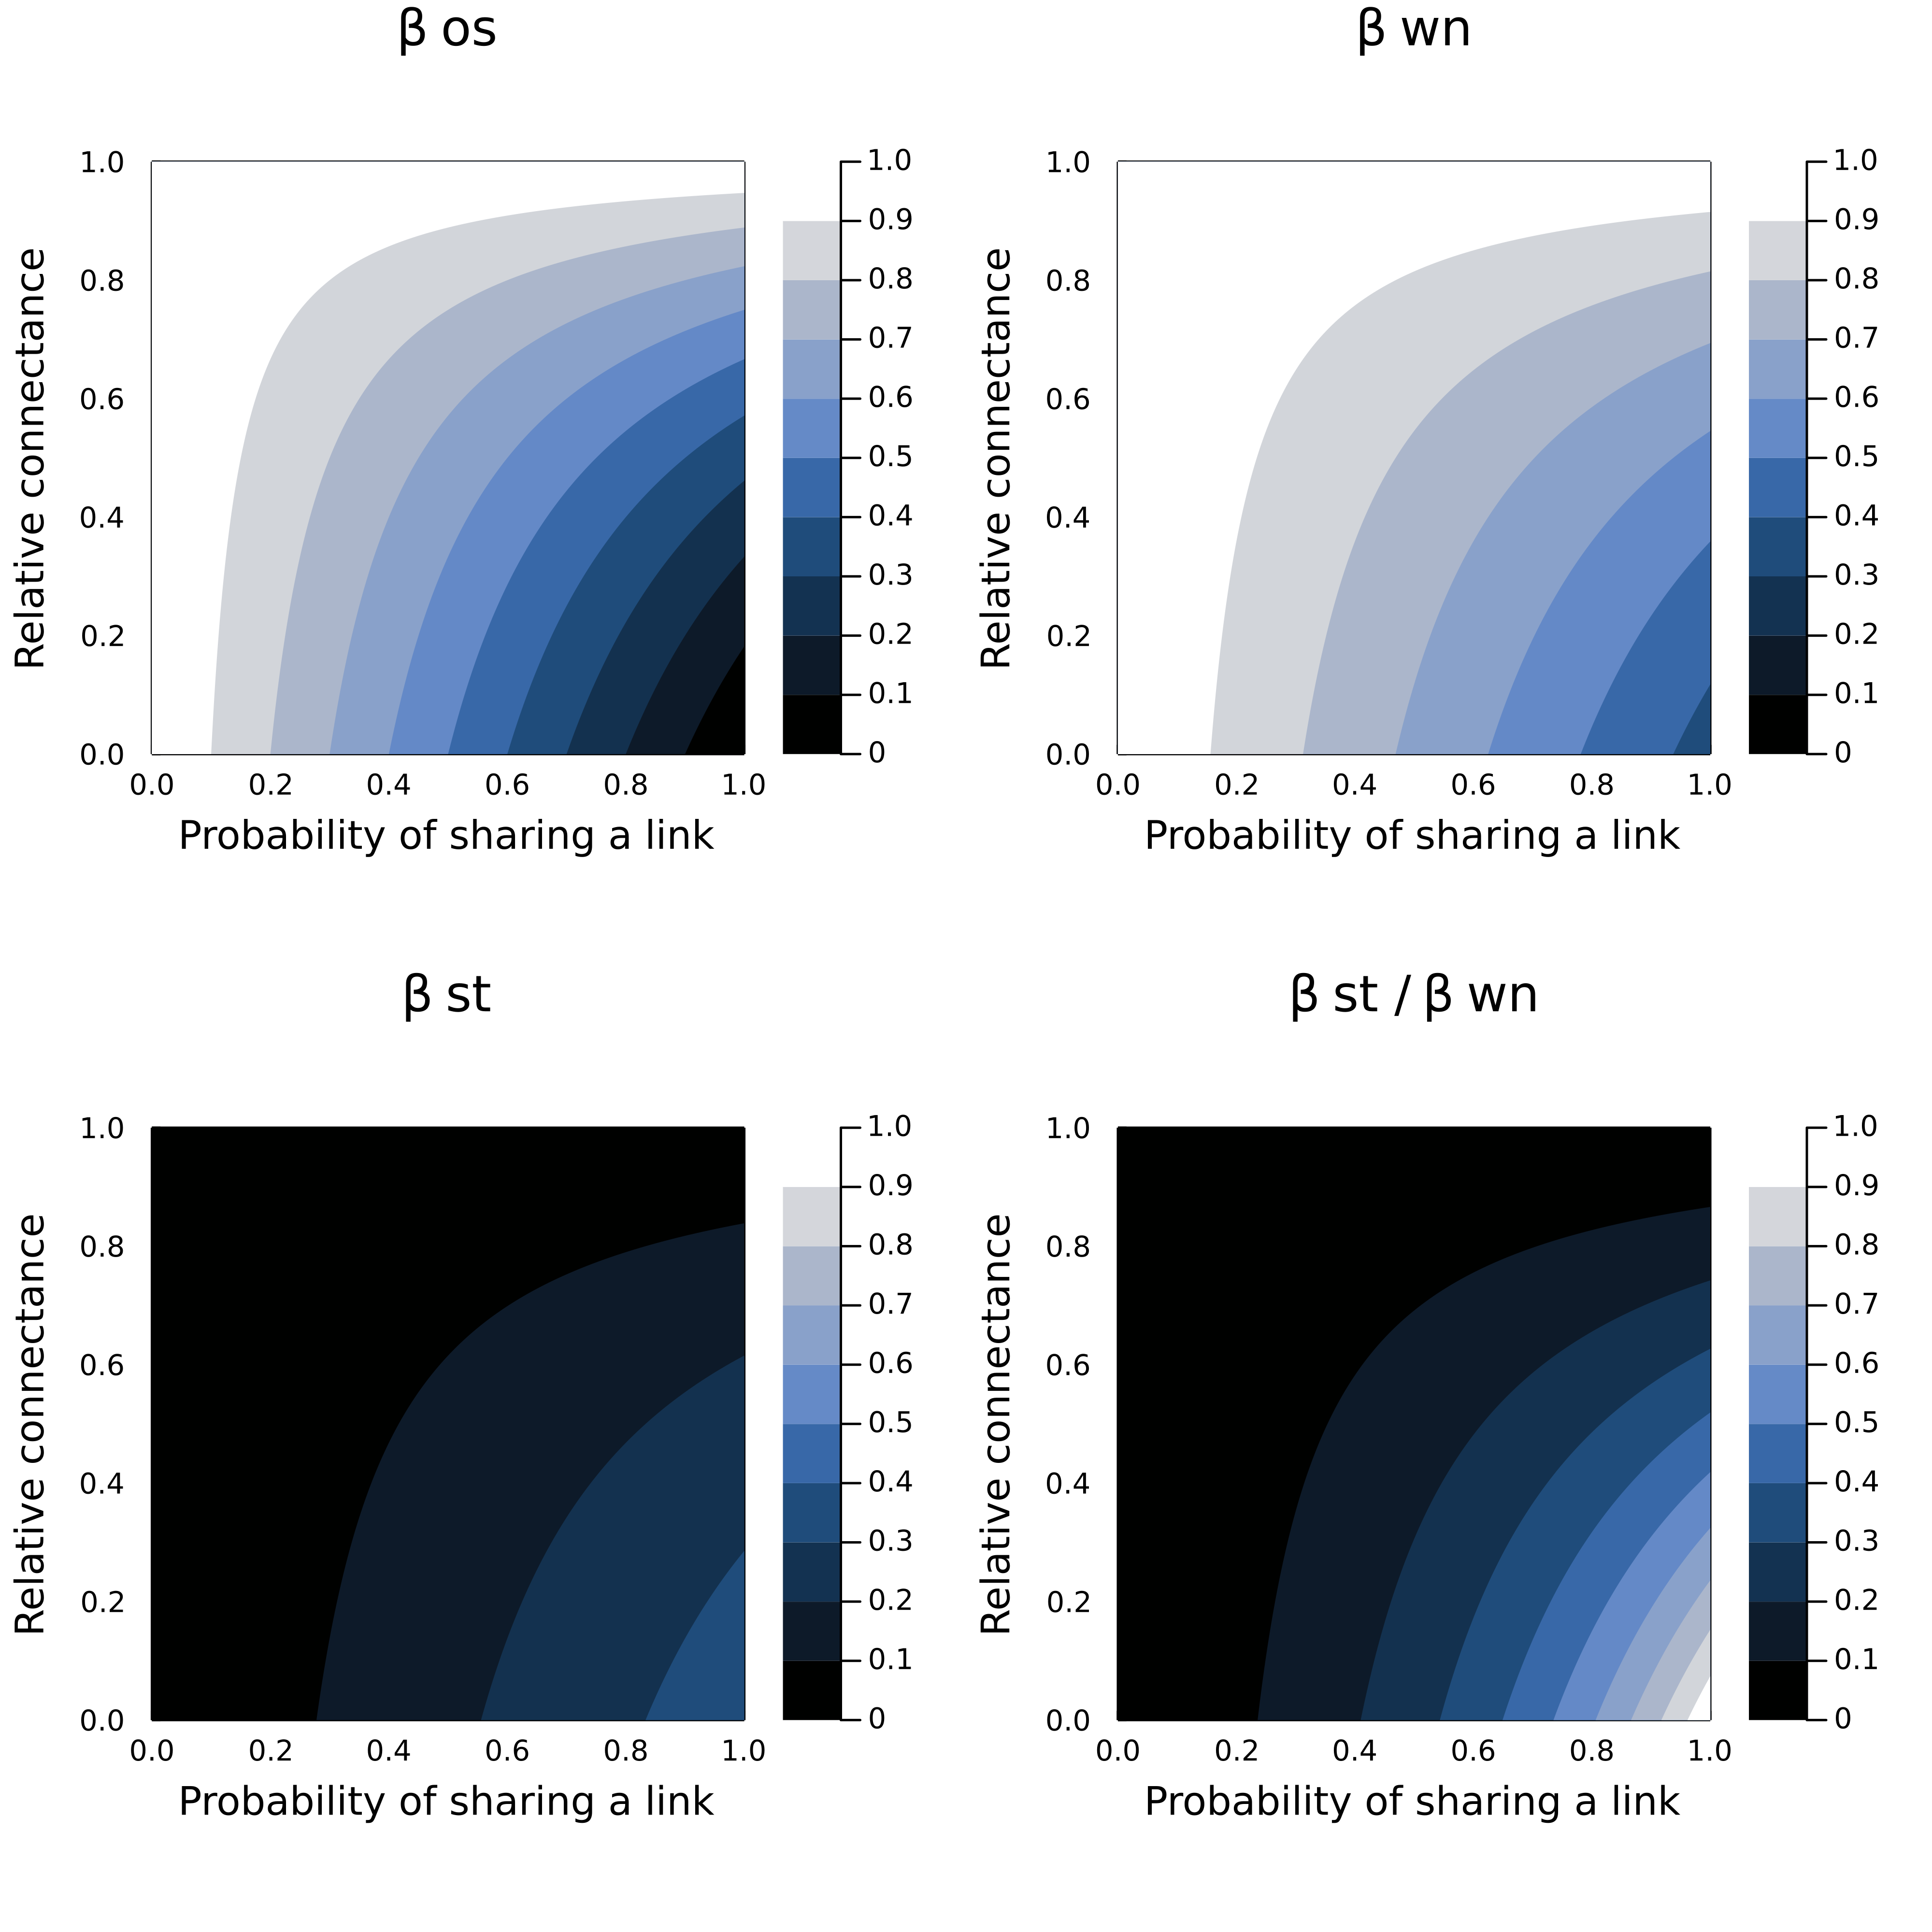
\includegraphics{figures/connectance/components.png}
\caption{Consequences of changing the ratio of connectances between two
equally species-rich networks on the decomposition of network
beta-diversity, assuming \(p = 0.8\). Networks with stronger differences
in connectance will tend to be more similar, because the differences in
number of links becomes extreme enough that the chances of all the links
in the sparser network being in the denser network
increases.}\label{fig:connectance}
}
\end{figure}

The values of these components are visualized in
fig.~\ref{fig:connectance}. The introduction of the connectance ratio
makes these expressions marginally more complex than in the case without
differences in connectance, but the noteworthy result remains that in
the presence of differences of connectance, the value of \(\beta_{os}\)
is still independent from species turnover. In fact, there is an
important conclusion to be drawn from this expression. The shared
species component is by definition square, meaning that from an actual
measurement of \(\beta_{os}\) between two networks for which we know the
connectance, noted \(\mathbf{b}_{os}\), we can get the probability of
rewiring by reorganizing the terms of
\(\mathbf{b}_{os} = 1 - 2aq/(1+a)\) as

\[q \approx \frac{(1-\mathbf{b}_{os})(a+1)}{2a}\,,\]

which gives the probability of rewiring as \(1-q\); note that this is an
\emph{approximation}, as it assumes that the connectances of the entire
network and the connectances of the shared components are the same.

\hypertarget{does-the-partition-of-network-dissimilarity-needs-a-new-normalization}{%
\subsection{Does the partition of network dissimilarity needs a new
normalization?}\label{does-the-partition-of-network-dissimilarity-needs-a-new-normalization}}

\hypertarget{is-this-decomposition-over-estimating-the-effect-of-rewiring}{%
\subsubsection{Is this decomposition over-estimating the effect of
``rewiring?''}\label{is-this-decomposition-over-estimating-the-effect-of-rewiring}}

One of the arguments put forth by Fründ (2021) is that the decomposition
outlined above will overestimate the effect of rewiring; I argue that
this is based on a misunderstanding of what \(\beta_{st}\) achieves. It
is paramount to clarify that \(\beta_{st}\) is not a direct measure of
the importance of turnover: it is a quantification of the relative
impact of rewiring to overall dissimilarity, which, all non-turnover
mechanisms being accounted for in the decomposition, can be explained by
turnover mechanisms. In this section, I present two numerical
experiments showing (i) that the \(\beta_{os}\) component is in fact an
accurate measure of rewiring, and (ii) that \(\beta_{st}\) captures the
consequences of species turnover, and of the interactions brought by
unique species.

\hypertarget{illustrations-on-arbitrarily-small-networks-are-biased}{%
\subsubsection{Illustrations on arbitrarily small networks are
biased}\label{illustrations-on-arbitrarily-small-networks-are-biased}}

We can re-calculate the illustration of Fründ (2021), wherein a pair of
networks with two shared interactions (\(A = 2\)) receive either an
interaction in \(S\), in \(U\), or in both:

\begin{longtable}[]{@{}lllllll@{}}
\toprule
\(A\) & \(S\) & \(U\) & \(\beta_{os}\) & \(\beta_{wn}\) & \(\beta_{st}\)
& \(\beta_{st}/\beta_{wn}\)\tabularnewline
\midrule
\endhead
2 & 0 & 0 & 0 & 0 & 0 &\tabularnewline
2 & 1 & 0 & \(1/5\) & \(1/5\) & 0 & 0\tabularnewline
2 & 0 & 1 & 0 & \(1/5\) & \(1/5\) & 0\tabularnewline
2 & 1 & 1 & \(1/5\) & \(1/3\) & \(2/15\) & \(2/5\)\tabularnewline
\bottomrule
\end{longtable}

The over-estimation argument hinges on the fact that
\(\beta_{st} < \beta_{os}\) in the last situation (one interaction as
rewiring, one as turnover). Reaching the conclusion of an overestimation
from this is based on a mis-interpretation of what \(\beta_{st}\) means.
The correct interpretation is that, out of the entire network
dissimilarity, only three-fifths are explained by re-wiring. The fact
that this fraction is not exactly one-half comes from the fact that the
Wilson \& Shmida (1984) measure counts shared interactions \emph{twice}
(\emph{i.e.} it has a \(2A\) term), which over-amplifies the effect of
shared interactions as the network is really small. Running the same
calculations with \(A = 10\) gives a relative importance of the turnover
processes of 47\%, and \(\beta_{st}\) goes to \(1/2\) as \(A/(S+U)\)
increases. As an additional caveat, the value of \(\beta_{st}\) will
depend on the measure of beta-diversity used. Measures that do not count
the shared interaction twice are not going to amplify the effect of
rewiring.

Based on the arguments presented above, I do not think the suggestion of
Fründ (2021) to change the denominator of \(\beta_{os}\) makes sense as
a default; the strength of the original approach by Poisot \emph{et al.}
(2012) is indeed that the effect of turnover is based on a rigorous
definition of networks as graphs (as opposed to networks as matrices),
in which the induction of vertices from the edgelist being compared
gives rise to biologically meaningful denominators. The advantage of
this approach is that at no time does the turnover of species itself (or
indeed, as shown in many places in this manuscript, the network
richness), or the connectance of the network, enter into the
calculation. As such, it is possible to use \(\beta_{os}\) and
\(\beta_{wn}\) in relationship to these terms, calculated externally (as
was recently done by \emph{e.g.} Higino \& Poisot 2021), without
creating circularities.

\textbf{TK} Therefore the argument of Fründ (2021), whereby the
\(\beta_{os}\) component should decrease with turnover, and be invariant
to connectance, does not hold: the very point of the approach is to
provide measures that can be interpreted in the light of connectance and
species turnover.

\textbf{TK} Adopting the perspective developed in the previous section,
wherein networks are sets and the measures of \(\beta\)-diversity
operates on these sets, highlights the conceptual issue in the Fründ
(2021) alternative normalization: they are using components of the
networks that are \emph{not} part of the networks being compared.

\hypertarget{numerical-experiment-the-decomposition-captures-the-roles-of-species-turnover-and-connectance-accurately}{%
\subsubsection{Numerical experiment: the decomposition captures the
roles of species turnover and connectance
accurately}\label{numerical-experiment-the-decomposition-captures-the-roles-of-species-turnover-and-connectance-accurately}}

Consider now two bipartite networks, which still have \(R\) species on
either side, but differ in their connectance (\(\rho_1\) and \(\rho_2\))
-- by maintaining the assumption that species on one side are shared
with probability \(p\), and that interactions between shared species are
rewired at probability \(q\), we can examine the effect of varying both
connectance and turnover on the value of the \(\beta\)-diversity
components. Note that, although not presented, we will drop the
multiplicative constant \(R^2\) from all calculations, as it is a common
factor for all values; again, this implies that the results presented
here are independant of network richness.

The number of unique links due to species turnover is

\[U = (1-p)(\rho_1 + \rho_2)\,,\]

which decreases with the proportion of shared species, but increases
with connectance. The number of links between shared species takes a
little more steps to calculate. First, amongst the \(pR^2\) species in
both sub-graphs, network 1 will have \(\rho_1 pR^2\), and network 2 will
have \(\rho_2 pR^2\). Because \(\rho_1 \neq \rho_2\), there are only
\(\text{min}(\rho_1, \rho_2)pR^2\) links that can be shared, a
proportion \(q\) of which will undergo re-wiring, and a proportion
\((1-q)\) of which will be shared. This leads to the expression (after
dropping \(R^2\)) for the number of shared links:

\[A = p (1-q) \text{min}(\rho_1, \rho_2)\,.\]

The number of unique links due to shared species is the sum of all links
in network 1 (\(\rho_1 R^2\)), minus the sum of the shared links
(\(AR^2\)) and the unique links due to species turnover
(\((1-p)\rho_1R^2\)); this same quantity is calculated in the same way
for the second networks, leading to (after dropping the multiplicative
constant \(R^2\) and some simplifications)

\[S = p (\rho_1 + \rho_2) - 2A\,.\]

Note that as expected, this last quantity scales with the proportion of
shared species (\(p\)) \emph{and} with connectance (as shared species
bring more of their interactions), but decreases with the size of the
shared links components. The consequences of varying \(\rho_2\) and
\(p\) are presented in fig.~\ref{fig:numexp3}.

\begin{figure}
\hypertarget{fig:commden}{%
\centering
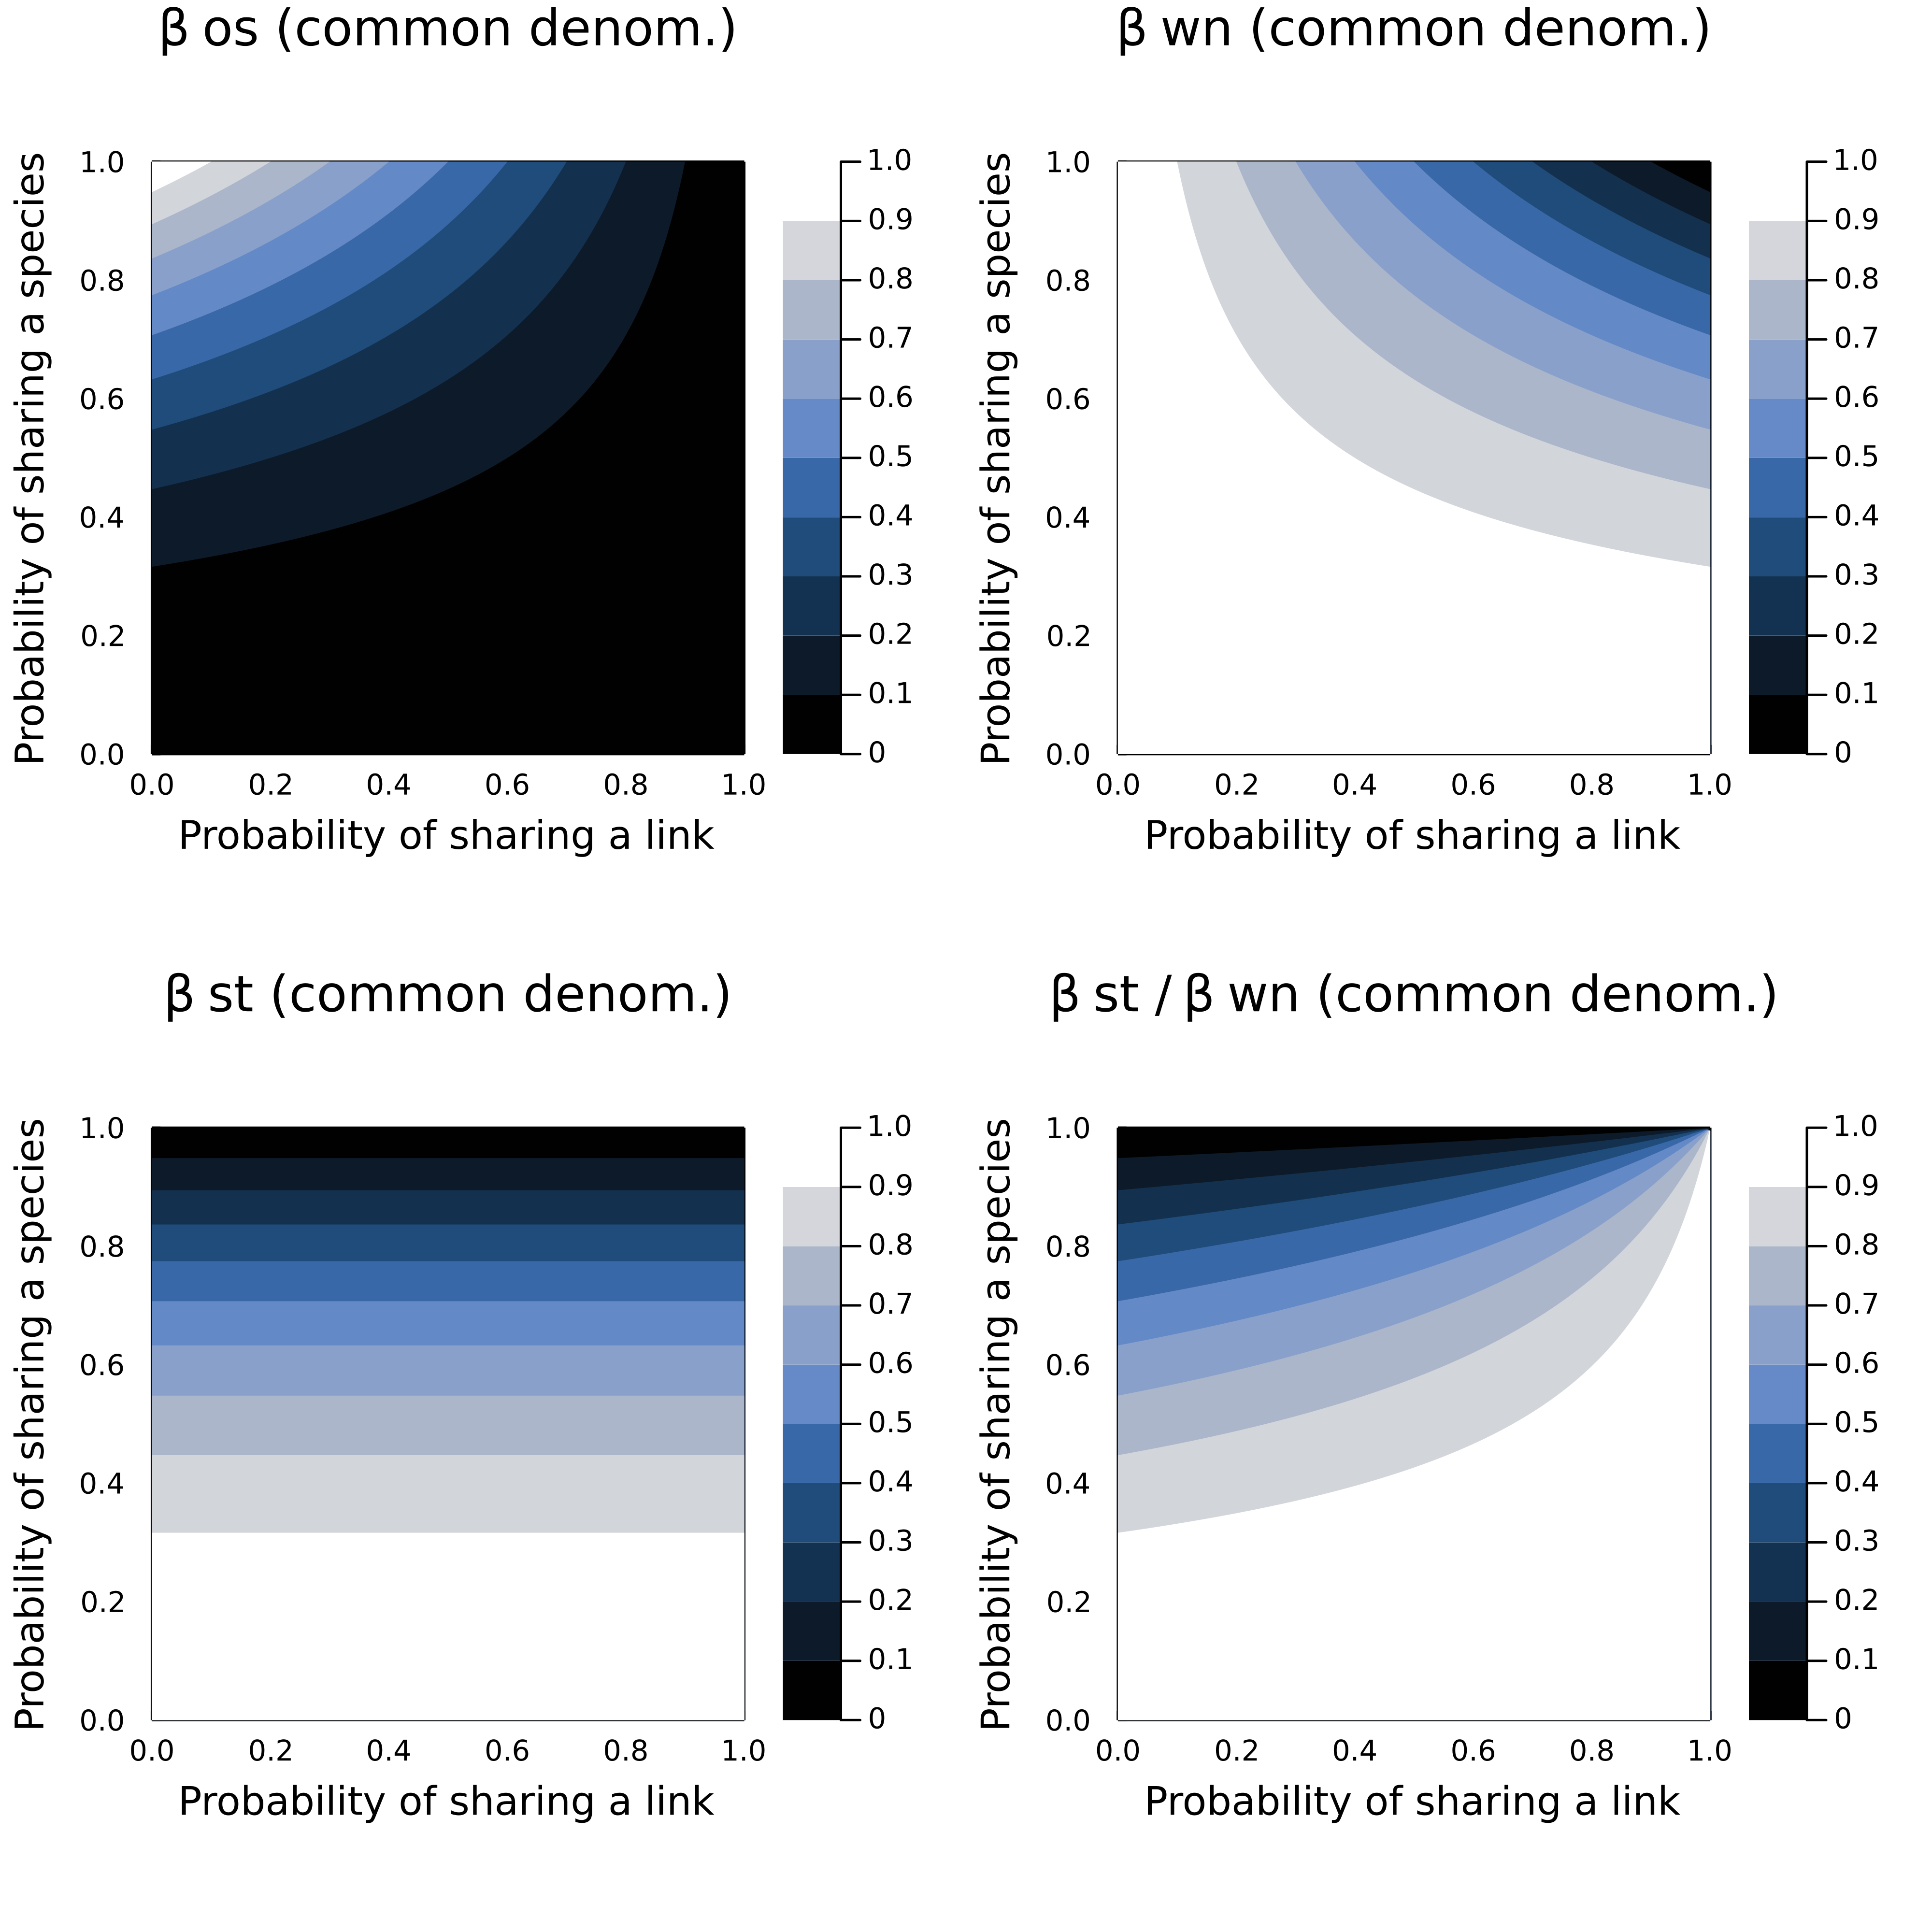
\includegraphics{figures/common_denominator/components.png}
\caption{Effects of varying the connectance of the second network
(\(\rho_2\)) and the proportion of shared species (\(p\)) on the values
of the \(\beta\)-diversity components. As expected, \(\beta_{os}\) is
still independent of species turnover, and \(\beta_{wn}\) increases when
species turnover increases, or when the connectances become more
dissimilar. These figures have been generated with \(\rho_1 = 0.25\) and
\(q = 0.15\), and the results are qualitatively robust to changes in
these parameters.}\label{fig:commden}
}
\end{figure}

Although \(\beta_{os}\) is only responding to changes in connectance (as
is expected, seeing that the relative connectances of both networks
appear in the expression for \(S\) and \(A\)), \(\beta_{wn}\) changes in
response to both parameters. Specifically, increasing the difference in
connectance between the two networks, especially when also increasing
the species dissimilarity, results in more dissimilar networks -- this
is because unique species from both networks bring their own
interactions (at rate \(\rho_1\) and \(\rho_2\)), and therefore
contribute to dissimilarity. It is particularly noteworthy that
\(\beta_{st}\), regardless of the differences in connectance, increases
with the proportion of unique species. At an equal proportion of shared
species, \(\beta_{st}\) \emph{decreases} with differences in
connectance: this is an equally expected result, which indicates that
the difference between \(\beta_{os}\) and \(\beta_{wn}\) is in part
explained by non-turnover mechanisms (here, changes in connectance).
Relying on the \(\beta_{st}/\beta_{wn}\) correction again magnifies this
effect, without changing their interpretation.

\hypertarget{measuring-network-beta-diversity-recommendations}{%
\subsection{Measuring network beta-diversity:
recommendations}\label{measuring-network-beta-diversity-recommendations}}

The choice of changing the denominator hinges on what one admits as a
definition for \(\beta_{st}\). If the point of \(\beta_{st}\) is to be a
component of overall \(\beta\)-diversity as advocated by Fründ (2021)
and Novotny (2009), a change of numerator \emph{might} be acceptable.
Nevertheless, this change of numerator contributes to blurring the
frontier between a measure of interaction dissimilarity and a measure of
community dissimilarity which starts to add the effect of relative
richness; this later case warrants a thorough methodological assessment.
Conversely, if as we argue in Poisot \emph{et al.} (2012),
\(\beta_{st}\) is to be meant as a \emph{guide} to the interpretation of
\(\beta_{wn}\) and \(\beta_{os}\), and related to actual measures of
species turnover and network connectance, one must not change the
denominator.

It is essential to recognize that there are multiple reasons to
calculate network dissimilarity, and it is our opinion that the
arguments levied by Fründ (2021) against the original partition stem
from a misunderstanding of what it intends to do (and does, indeed, do
well), not from intrinsic methodological issues in the partition itself.
Based on the results presented in this contribution, I argue that the
original partition of network \(\beta\)-diversity from Poisot \emph{et
al.} (2012) should remain the default.

\hypertarget{references}{%
\subsection*{References}\label{references}}
\addcontentsline{toc}{subsection}{References}

\hypertarget{refs}{}
\begin{CSLReferences}{1}{0}
\leavevmode\hypertarget{ref-Baronio2021NatFir}{}%
Baronio, G.J., Souza, C.S., Maruyama, P.K., Raizer, J., Sigrist, M.R. \&
Aoki, C. (2021). Natural fire does not affect the structure and beta
diversity of plant-pollinator networks, but diminishes floral-visitor
specialization in Cerrado. \emph{Flora}, 281, 151869.

\leavevmode\hypertarget{ref-Campos-Moreno2021ImpInt}{}%
Campos-Moreno, D.F., Dyer, L.A., Salcido, D., Massad, T.J.,
Pérez-Lachaud, G., Tepe, E.J., \emph{et al.} (2021). Importance of
interaction rewiring in determining spatial and temporal turnover of
tritrophic (Piper-caterpillar-parasitoid) metanetworks in the Yucatán
Península, México. \emph{Biotropica}, 53, 1071--1081.

\leavevmode\hypertarget{ref-Canard2014EmpEva}{}%
Canard, E.F., Mouquet, N., Mouillot, D., Stanko, M., Miklisova, D. \&
Gravel, D. (2014). Empirical evaluation of neutral interactions in
host-parasite networks. \emph{The American Naturalist}, 183, 468--479.

\leavevmode\hypertarget{ref-Dunne2006NetStr}{}%
Dunne, J.A. (2006). The Network Structure of Food Webs. In:
\emph{Ecological networks: Linking structure and dynamics} (eds. Dunne,
J.A. \& Pascual, M.). Oxford University Press, pp. 27--86.

\leavevmode\hypertarget{ref-Frund2021DisSpe}{}%
Fründ, J. (2021). Dissimilarity of species interaction networks: How to
partition rewiring and species turnover components. \emph{Ecosphere},
12, e03653.

\leavevmode\hypertarget{ref-Higino2021BetPhy}{}%
Higino, G.T. \& Poisot, T. (2021). Beta and phylogenetic diversities
tell complementary stories about ecological networks biogeography.
\emph{Parasitology}, 1--23.

\leavevmode\hypertarget{ref-Koleff2003MeaBet}{}%
Koleff, P., Gaston, K.J. \& Lennon, J.J. (2003). Measuring beta
diversity for presence--absence data. \emph{Journal of Animal Ecology},
72, 367--382.

\leavevmode\hypertarget{ref-Legendre2013BetDiv}{}%
Legendre, P. \& De Cáceres, M. (2013). Beta diversity as the variance of
community data: Dissimilarity coefficients and partitioning.
\emph{Ecology Letters}, 16, 951--963.

\leavevmode\hypertarget{ref-Magrach2017PlaNet}{}%
Magrach, A., Holzschuh, A., Bartomeus, I., Riedinger, V., Roberts,
S.P.M., Rundlöf, M., \emph{et al.} (2017). Plant-pollinator networks in
semi-natural grasslands are resistant to the loss of pollinators during
blooming of mass-flowering crops. \emph{Ecography}, n/a--n/a.

\leavevmode\hypertarget{ref-Novotny2009BetDiv}{}%
Novotny, V. (2009). Beta diversity of plant--insect food webs in
tropical forests: A conceptual framework. \emph{Insect Conservation and
Diversity}, 2, 5--9.

\leavevmode\hypertarget{ref-Olsson2021IntPla}{}%
Olsson, R.L., Brousil, M.R., Clark, R.E., Baine, Q. \& Crowder, D.W.
(2021). Interactions between plants and pollinators across urban and
rural farming landscapes. \emph{Food Webs}, 27, e00194.

\leavevmode\hypertarget{ref-Poisot2012DisSpe}{}%
Poisot, T., Canard, E., Mouillot, D., Mouquet, N. \& Gravel, D. (2012).
The dissimilarity of species interaction networks. \emph{Ecology
Letters}, 15, 1353--1361.

\leavevmode\hypertarget{ref-Poisot2016StrPro}{}%
Poisot, T., Cirtwill, A.R., Cazelles, K., Gravel, D., Fortin, M.-J. \&
Stouffer, D.B. (2016). The structure of probabilistic networks.
\emph{Methods in Ecology and Evolution}, 7, 303--312.

\leavevmode\hypertarget{ref-Poisot2017HosPar}{}%
Poisot, T., Gueveneux-Julien, C., Fortin, M.-J., Gravel, D. \& Legendre,
P. (2017). Hosts, parasites and their interactions respond to different
climatic variables. \emph{Global Ecology and Biogeography}, n/a--n/a.

\leavevmode\hypertarget{ref-Poisot2015SpeWhy}{}%
Poisot, T., Stouffer, D.B. \& Gravel, D. (2015). Beyond species: Why
ecological interaction networks vary through space and time.
\emph{Oikos}, 124, 243--251.

\leavevmode\hypertarget{ref-Souza2021PlaSam}{}%
Souza, C.S., Maruyama, P.K., Santos, K.C.B.S., Varassin, I.G., Gross,
C.L. \& Araujo, A.C. (2021). Plant-centred sampling estimates higher
beta diversity of interactions than pollinator-based sampling across
habitats. \emph{New Phytologist}, 230, 2501--2512.

\leavevmode\hypertarget{ref-Trojelsgaard2016EcoNet}{}%
Trøjelsgaard, K. \& Olesen, J.M. (2016). Ecological networks in motion:
Micro- and macroscopic variability across scales. \emph{Functional
Ecology}, 30, 1926--1935.

\leavevmode\hypertarget{ref-Tuomisto2010DivBet}{}%
Tuomisto, H. (2010). A diversity of beta diversities: Straightening up a
concept gone awry. Part 1. Defining beta diversity as a function of
alpha and gamma diversity. \emph{Ecography}, 33, 2--22.

\leavevmode\hypertarget{ref-Wilson1984MeaBet}{}%
Wilson, M.V. \& Shmida, A. (1984). Measuring Beta Diversity with
Presence-Absence Data. \emph{Journal of Ecology}, 72, 1055--1064.

\end{CSLReferences}

\end{document}
